\begin{figure}[t]
\centering
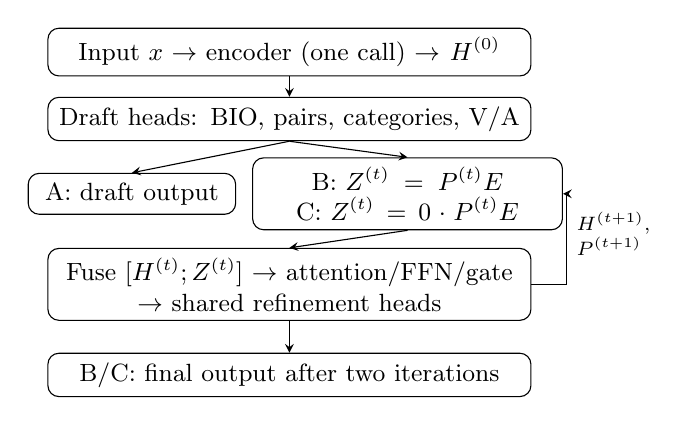
\begin{tikzpicture}[>=stealth, every node/.style={font=\small}, box/.style={draw,rounded corners,align=center,text width=5.9cm,minimum height=0.52cm}]
\node[box] (enc) at (0,0) {Input $x$ $\rightarrow$ encoder (one call) $\rightarrow H^{(0)}$};
\node[box] (draft) at (0,-0.85) {Draft heads: BIO, pairs, categories, V/A};
\node[box,text width=2.4cm] (a) at (-2,-1.8) {A: draft output};
\node[box,text width=3.7cm] (bc) at (1.5,-1.8) {B: $Z^{(t)}=P^{(t)}E$\\C: $Z^{(t)}=0\cdot P^{(t)}E$};
\node[box] (refine) at (0,-2.95) {Fuse $[H^{(t)};Z^{(t)}]$ $\rightarrow$ attention/FFN/gate\\$\rightarrow$ shared refinement heads};
\node[box] (out) at (0,-4.1) {B/C: final output after two iterations};
\draw[->] (enc)--(draft);
\draw[->] (draft.south)--(a.north);
\draw[->] (draft.south)--(bc.north);
\draw[->] (bc.south)--(refine.north);
\draw[->] (refine)--(out);
\draw[->] (refine.east)--++(0.45,0)|-node[pos=0.28,right,font=\scriptsize,align=left] {$H^{(t+1)}$,\\$P^{(t+1)}$} (bc.east);
\end{tikzpicture}
\caption{Active inference paths. B/C repeat the refinement block twice with shared weights. Only BIO predictions feed token refinement; the computed pair-fusion output is discarded. A bypasses refinement.}
\label{fig:feedback}
\end{figure}
